\documentclass[spanish, fleqn]{article}
\usepackage[english]{babel}
\usepackage[utf8]{inputenc}
\usepackage{amsmath}
\usepackage{amsfonts}
%\usepackage{wasysym}
%\usepackage{mathrsfs}
\usepackage[colorlinks, urlcolor=blue]{hyperref}
\usepackage[top = 2.5cm, bottom = 2cm, left = 2.5cm, right = 2.5cm]{geometry}
\usepackage{fancyhdr, graphicx}
\usepackage{caption}

\usepackage{changepage}
\usepackage{wrapfig}

\renewcommand{\headrulewidth}{0pt}
\fancyhead[L]{
\includegraphics[width=3cm]{Logo_INFO.png}}
\fancyhead[R]{
\includegraphics[width=3.2cm]{Logo_UTFSM.png}}


\title{ La ética nacional.}
\author{Hernán Vargas, 201073009-3 \\ hernan.vargas@alumnos.usm.cl}
\date{\today}

\begin{document}
	\maketitle
	\thispagestyle{empty}
%	\newpage
%	\null
%	\vskip 4em
%	\begin{center}
%		\textsc{\Large Universidad Técnica Federico Santa María.}\\[0.4cm]
%		\textsc{\Large Sistemas y Organizaciones.}\\[0.2cm]
%		\textsc{\LARGE Análisis de la Estructura Organizacional.}\\[1.2cm]
%	\end{center}

	\thispagestyle{fancy}
	\section{Ética en el siglo de los cambios.}
	Sin duda vivimos en una época de grandes cambios, las tecnologías de la
	información y comunicación han creado las bases de la vida en el siglo XXI.
	Nos ayudan prácticamente en toda labor que efectuemos pero, a pesar de esto,
	también nos encaminan hacia nuevos desafíos y nos hacen vislumbrar nuevos
	problemas. En este ambiente algunos hombres pierden el camino, comienzan a 
	ser consientes de dificultades que antes ignoraban y esta situación los pone
	intranquilos y merma su capacidad de razonar correctamente.\\
	Son estos dilemas éticos los que se discutirán en esté informe. Dichos
	dilemas generalmente son referentes a temas complejos, situaciones en las
	cuales no podemos saber que es lo `bueno', lo `justo' o lo `apropiado'.\\
	A la hora de enfrentar estos problemas, tenemos que tener en cuenta algunos
	factores que condicionarán nuestro actuar. En primer lugar, no existen
	soluciones perfectas, cada acción tiene su reacción, y por ello, nuestras
	medidas tendrán resultados tanto beneficiosos como perjudiciales.\\
	En segundo lugar, no podemos evitar tener sesgos, ya sean intelectuales, 
	sociales o culturales, estamos supeditados a ellos y es por esto que
	nuestras decisiones serán en gran parte influenciadas. Entonces, 
	¿Como podemos tomar buenas decisiones en temas éticos? La respuesta no es
	simple, pero al menos debemos considerar los factores antes descritos además
	del constante auto-cultivo de virtudes y saber diferencial que es lo más
	conveniente para una organización.
	
	\section{Dilemas éticos de una organización.}
	El artículo nos muestra que una organización, en esté caso una 
	empresa con fines comerciales, debe estar consiente de al menos los
	siguientes cinco dilemas que le afectan:\\
	\begin{minipage}{0.6\textwidth}
	\begin{enumerate}
		\item \textbf{Liderazgo ético:}
			La correcta apreciación del sentido de la autoridad y el poder.
		\item \textbf{Relación empresa-trabajador:}
			Los nuevos tiempos pasaron la relación de la lealtad al beneficio
			mutuo.
		\item \textbf{(Des)equilibrio del trabajo-familia:}
			Las largas jornadas de trabajo y la inserción de la mujer al mundo 
			laboral ha cambiado la antigua idea de como debe ser una familia.
		\item \textbf{Educación y pobreza:}
			La contingencia y relevancia del tema no lo hace solo
			responsabilidad del estado, las demás organizaciones también deben
			ser conscientes de como se ven afectadas por ello.
		\item \textbf{Medio ambiente:}
			Hoy en día toda organización debe ser responsable con su medio
			ambiente, la carga social por ello no debe ser ignorada.
	\end{enumerate}
	\end{minipage}
	\hfill
	\begin{minipage}{0.4\textwidth}
    	\begin{center}
			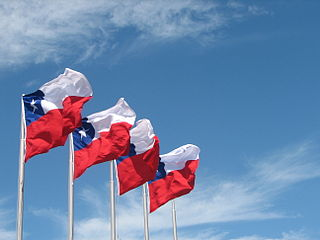
\includegraphics[width=0.9\textwidth]{chile_flag.jpg}
	    	Banderas de Chile\cite{r2} flameando al viento, un claro recuerdo
			del ambiente que envuelve al país este mes.
		\end{center}
	\end{minipage}

	\newpage
	\newgeometry{left=2.5cm, right=2.5cm, top=2.5cm, bottom=2.5cm}
	\section{Decisiones éticas en septiembre.}
	El mes de septiembre es un periodo bastante delicado para todo chileno, se 
	celebran y recuerdan hechos que hasta hoy en día tiene repercusiones, tanto
	económicas como políticas y sociales. Este 9 de septiembre, se 
	\emph{celebraba} en isla de pascua su anexión al territorio nacional con
	protestas contra el estado chileno\cite{r3}, se esperan manifestaciones y 
	disturbios para este 11 de septiembre, aniversario del golpe de estado de
	1972 y la próxima semana será nuestras ansiadas fiestas patrias. En medio 
	de este caótico clima los noticiarios nos informaron sobre una situación
	pocas veces vistas en Chile: los atentados con bombas en el metro\cite{r4},
	en supermercados\cite{r5} y por si fuera poco, la dudosa fabricación de 
	bombas en un colegio de santiago\cite{r6}.\\
	Pero, ¿Qué tienen que ver estos hechos con las decisiones éticas?, simple, 
	todas estas situaciones están basadas en problemáticas complejas, en las 
	cuales no se puede tomar una decisión sin tener en cuenta las consecuencias.
	En este aspecto, considero que la mayoría de estas situaciones han sido en 
	parte ocasionadas o mal tratadas por el gobierno. El descontento de la gente
	suele explotar, en este caso literalmente, cuando no sienten que sus ideas
	y problemáticas son tratadas con el respeto que merecen. Los conflictos y 
	las protestas por temas como la educación, la generación de energía, la 
	desigualdad entre otros, eran parte habitual de nuestro día a día 
	últimamente, pero ahora, después de los supuestos terroristas del metro, se
	intentan apresurar de manera forzada las leyes que quitan libertades a la
	hora de protestar, movimiento que viene de la mano con una gran cobertura
	mediática. Que coincidencia. \\
	Por supuesto, si bien el gobierno de Chile ha errado a la hora de satisfacer
	las demandas en temas con profundas raíces éticas, este problema no solo se
	hace presente ahí. Muchas veces las marchas terminan en destrozos; El sujeto
	que pone la bomba, sin importar que motivo tuvo, erró en su decisión a la 
	hora de hacer notar su descontento.

	\section{Conclusiones.}
	Enseñar a enfrentar de buena manera los problemas éticos es difícil, en 
	parte por que gran parte de esto se resume al enriquecimiento personal,
	mientras que por otro lado tenemos que no existen decisiones acertadas. 
	Generalmente una solución en este ámbito traerá nuevos problemas, pero no
	por ello debemos cerrar los ojos ante las dificultades que nos presenta el
	futuro.

	\renewcommand{\refname}{\selectfont 5 \, Referencias} % Hack para nombre
	\begin{thebibliography}{x}
		\bibitem{r2}
			\textit{Chile flags in Puerto Montt} - Mark Scott Johnson, 
			\href{http://flickr.com/photos/39791353@N00}
			{http://flickr.com/photos/39791353@N00}
			revisado el 10 de septiembre del 2014.
		\bibitem{r3}
			\textit{Protesta contra Estado de Chile en Isla de Pascua} - 
			El Ciudadano, 
			revisado el 10 de septiembre del 2014:
			\href{http://www.elciudadano.cl/2014/09/09/114484/protesta-contra-estado-de-chile-en-isla-de-pascua/}
			{http://www.elciudadano.cl/2014/09/09/114484/protesta-contra-estado-de-chile-en-isla-de-pascua/}.
		\bibitem{r4}
			\textit{¿Quién pone bombas en Chile, uno de los países más seguros
			de Latinoamérica?} - Biobio Chile, 
			\href{http://www.biobiochile.cl/2014/09/10/quien-pone-bombas-en-chile-uno-de-los-paises-mas-seguros-de-latinoamerica.shtml}
			{http://www.biobiochile.cl/2014/09/10/quien-pone-bombas-en-chile-uno-de-los-paises-mas-seguros-de-latinoamerica.shtml},
			revisado el 10 de septiembre del 2014.
		\bibitem{r5}
			\textit{Un nuevo atentado con bomba en Chile} - 20minutos.es, 
			\href{http://www.20minutos.es/noticia/2234211/0/bomba-supermercado/persona-herida/chile/}
			{http://www.20minutos.es/noticia/2234211/0/bomba-supermercado/persona-herida/chile/},
			revisado el 10 de septiembre del 2014.
		\bibitem{r6}
			\textit{Encuentran 50 bombas molotov en un instituto de Chile} - elEconomista, 
			\href{http://www.eleconomistaamerica.cl/actualidad-eAm-chile/noticias/6068167/09/14/Encuentran-50-bombas-molotov-en-un-instituto-en-Chile.html}
			{http://www.eleconomistaamerica.cl/actualidad-eAm-chile/noticias/6068167/09/14/Encuentran-50-bombas-molotov-en-un-instituto-en-Chile.html},
			revisado el 10 de septiembre del 2014.

	\end{thebibliography}

	%Referencias.
	\begin{flushright}
		\textbf{Palabras clave:} \emph{Ética, Chile, protestas.}
		\begin{flalign*}
			&&\text{\textbf{Tiempo SCT}: \emph{Análisis del artículo}} &= 0:25 \\
										 &&\emph{Creación del informe} &= 2:27 \\
												&&\emph{Investigación} &= 0:50 \\
											            &&\text{Total} &= 3:42
		\end{flalign*}
	\end{flushright}

\end{document}
